\documentclass[12pt,a4paper,draft]{report}
\usepackage[utf8]{inputenc}
\usepackage[german]{babel}
\usepackage[T1]{fontenc}
\usepackage{amsmath}
\usepackage{amsfonts}
\usepackage{amssymb}
\usepackage{lmodern}
\usepackage{authoraftertitle}
\usepackage[final]{graphicx}
\DeclareGraphicsExtensions{.pdf,.png,.jpg}
\usepackage{color}

\definecolor{dkgreen}{rgb}{0,0.6,0}
\definecolor{gray}{rgb}{0.5,0.5,0.5}
\definecolor{mauve}{rgb}{0.58,0,0.82}

\date{29.09.2014}
\author{Ari Ayvazyan}
\title{State Machines}


\begin{document}
\maketitle

\tableofcontents

\chapter{Angabe}
Implement a component based C-Programm to show the difference of the 5 types of state machines presented in the book of Mrs. Elicia White "Making Embedded Systems" with traffic light system we discussed in the lesson. To test your implementation you can use simple output functions (e.g. fprintf), but be prepared to implement it also on hardware (GPIO with Leds, Timers, etc.).
\newline
Don't forget to document the differences (advantages/disadvantages) in your protocol.

\begin{figure}[h]
\centering
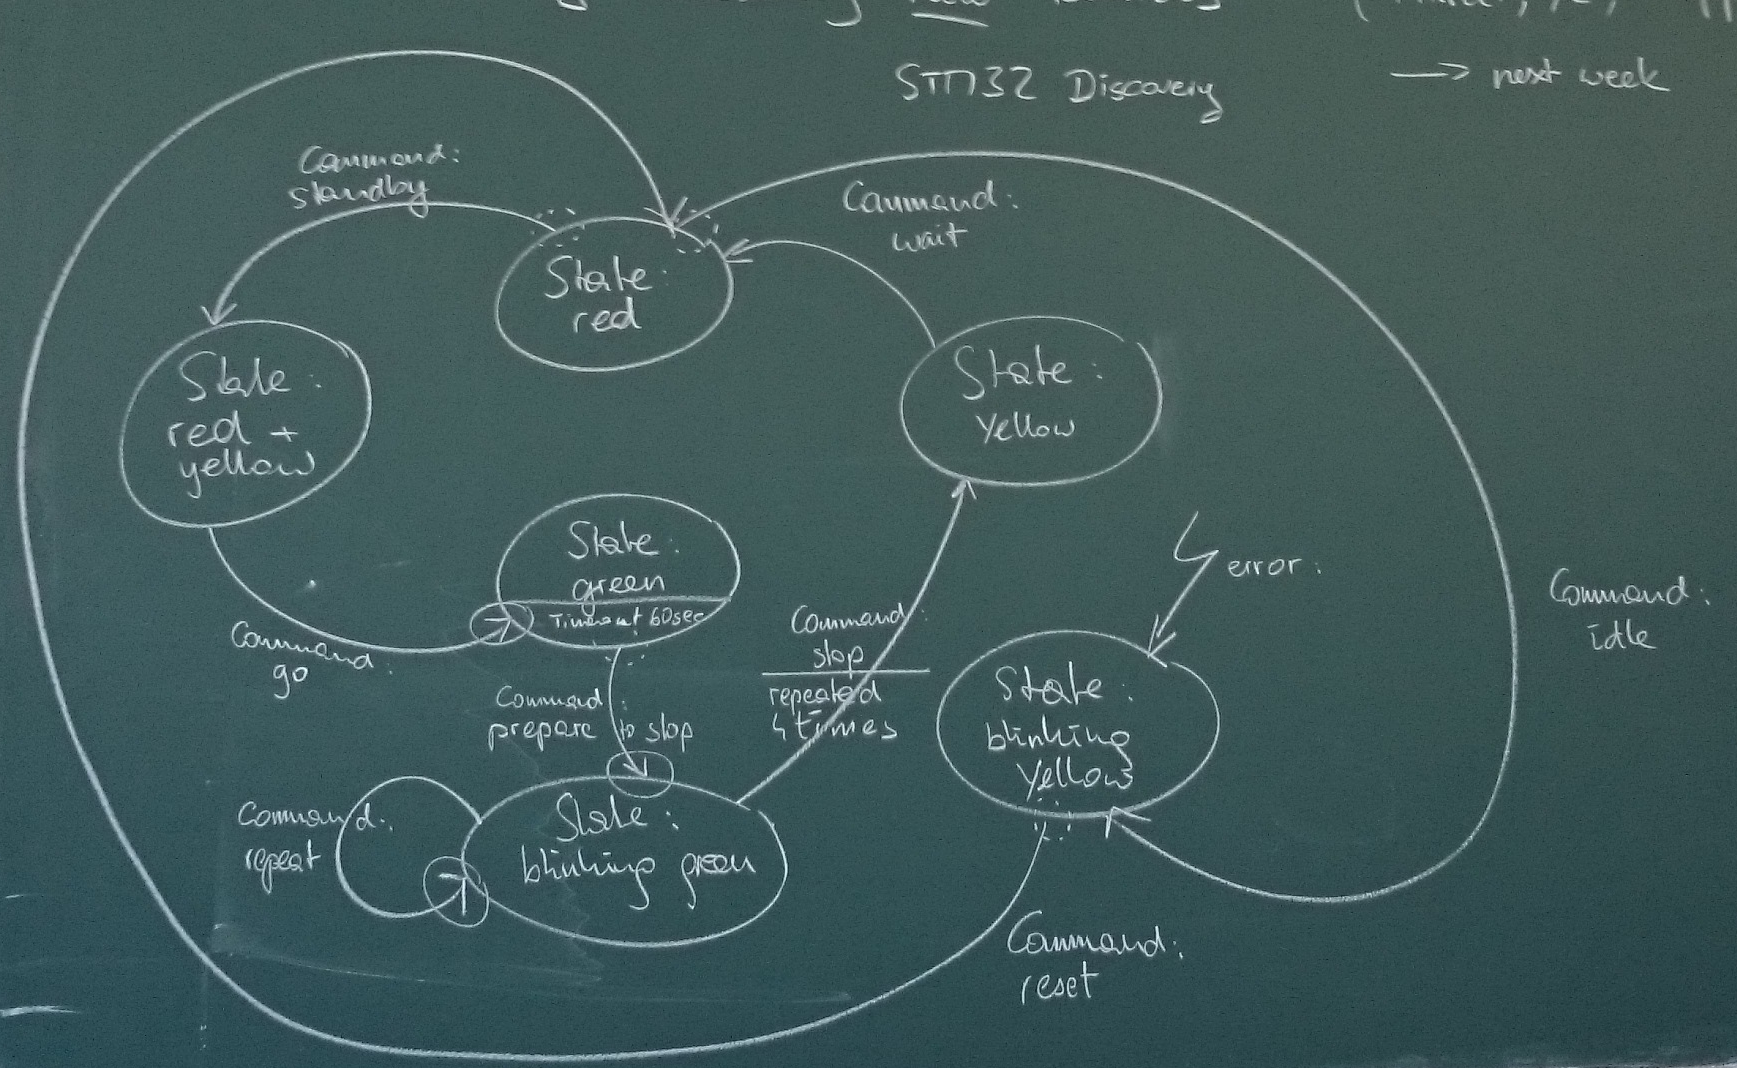
\includegraphics[width=1\linewidth]{angabeTafel.png}
\label{fig:angabeTafel}
\end{figure}

\chapter{Designüberlegung}

Umzusetzen sind folgende 5 State Machine Patterns:
\newline
\begin{enumerate}
	\item State Centric \newline
	Hier steht der Status im Vordergrund, es wird erst auf den Status geprüft und anschließend gecheckt welches Kommando zu diesem Status ausgeführt werden soll.
	\begin{verbatim}

	void trafficLight(TrafficLightState* state, Command *command) {
		switch(*state) {
			case Red:
			if(*command==Wait){
				
	\end{verbatim}
	\item State Centric Hidden \newline
	Hier steht ebenfalls der Status im Vordergrund, es wird erst auf den Status geprüft, dieser wird auch gesetzt und anschließend gecheckt welches Kommando zu diesem Status ausgeführt werden soll um Letztendlich via Separater Methode zu prüfen was als nächstes getan werden soll.  
	\begin{verbatim}
	
	switch(*state) {
	case Red:
	if(strcmp(currentTrafficLightColor,"Red")!=0) {
	strcpy(currentTrafficLightColor, "Red");
	outTrC(Red);
	}
	if(*command==Wait){
	
	\end{verbatim}
	\item Event Centric \newline
	Hier steht das Kommando im vordergrund, je nach Kommando wird anschließend auf den Status geprüft und dementsprechend gehandelt.
	\begin{verbatim}
	switch(*command) {
	case Standby:
	if(*state==RedYellow){
	strcpy(currentTrafficLightColor, "RedYellow");
	outTrC(RedYellow);
	Sleep(SLEEP_TIME);
	NEXTSTATE;
	}
	\end{verbatim}
	
	\item State Pattern \newline
	Hierbei handelt es sich um eine Objektorientierte Variante der State Machine.\newline
	Das State Objekt besitzt folgende Funktionen:\newline
	\begin{verbatim}
	Enter wird zu beginn eines states ausgeführt
	
	Exit wird beim verlassen eines states ausgeführt
	
	EventGo verarbeitet das go event
	
	EventStop verarbeitet das stop event
	
	Housekeeping prüft auf änderungen
	
	\end{verbatim}
	
	\item Table Driven \newline
	
\end{enumerate}

\chapter{Aufwandschätzung}


Schätzung: 10 Stunden\newline

Tatsächliche Zeit: 13 Stunden\newline

\chapter{Durchführung}
Es wurde anhand der zur Verfügung gestellten Ressourcen geforscht welche State Machines Existieren und wie diese umzusetzen sind.\newline

\section{Probleme}
\subsection{LaTeX}
LaTeX zeigte sich anfangs durch Variablen und Format-freie Schreibfläche von seiner schönen Seite, jedoch ging einiges an Zeit an der Fehlerbehebung verloren:
\subsubsection{Bilder}Bilder wurden im Editor nicht angezeigt, dies ließ sich nach Zeitaufwendiger Recherche durch setzen der Option final bei: 
\begin{verbatim}
\usepackage[final]{graphicx}
\end{verbatim}
beheben.
\newpage
\subsection{Farbdarstellung}
Die Farbdarstellung war eine Herausforderung, sie ist unter Linux Systemen einfach mittels ANSI Formatierung möglich, jedoch unterstützt Windows dies seit Windows NT nicht mehr. \newline Unter Windows bietet \begin{verbatim}
windows.h
\end{verbatim} eine Möglichkeit zur Änderung der Text und Hintergrundfarbe. \newline
Leider ließ sich das Problem nur über Umwege mithilfe eines System abhängiges \#ifdef... \#define lösen. \newline
Eine Intensive Recherche führte zu lediglich einer in C geschriebenen Library: ncurses.
Diese war via apt-get vor dem compilieren zu installieren, ist jedoch auch zum Download verfügbar.\newline
Es stellte sich heraus das die Library für diese übung ein Overkill ist und etwas anderes her musste. \newline
Die Lösung wurde in cfprintf.c realisiert. Hier wird je nach verwendetem Betriebssystem die entsprechende Funktion zur Darstellung der Farbe gewählt. ANSI sowie die windows.h funktionen


\chapter{Installationsanleitung}
Via CMake -i kann ein Makefile mit Build Konfigurationen für jede State Machine erstellt werden.\newline
Diese wird mit make target aufgerufen


\end{document}